%!TEX root=document.tex


\section{{\large \SeeDB\ } Design}
\label{sec:system_architecture}

In this section, we present an overview of the \SeeDB\ architecture.
\SeeDB\ is comprised of two main parts: the frontend and the backend. 
The \SeeDB\ frontend is a ``thin client''
that is used to issue queries, display visualizations and allow basic interactions
with the visualizations. 
The backend, in contrast, performs all the computation required to generate and select views
to be recommended. 
Figure \ref{fig:sys-arch} depicts the architecture of our system.
Once the analyst issues a query via the frontend, the backend takes over.
First, the View Generator queries the system metadata for information such as
table sizes, column types, correlations between column values etc. 
It then uses this metadata and the incoming query to prune the space
of possible views and generate stubs for the remaining views. 
View stubs are essentially more elaborate triples of the form $(a, m, f)$ as
discussed in Section \ref{}. 
The generated view stubs are then sent to the Execution Engine that is
responsible for querying the underlying data, evaluating the utility of each
candidate view, and identifying the top views of interest. 
Once the \SeeDB\ backend has identified the best views, the \SeeDB\
frontend generates and displays visualizations for each of these views. 

\begin{figure}[htb]
\vspace{-10pt}
\centerline{
\hbox{\resizebox{9cm}{!}{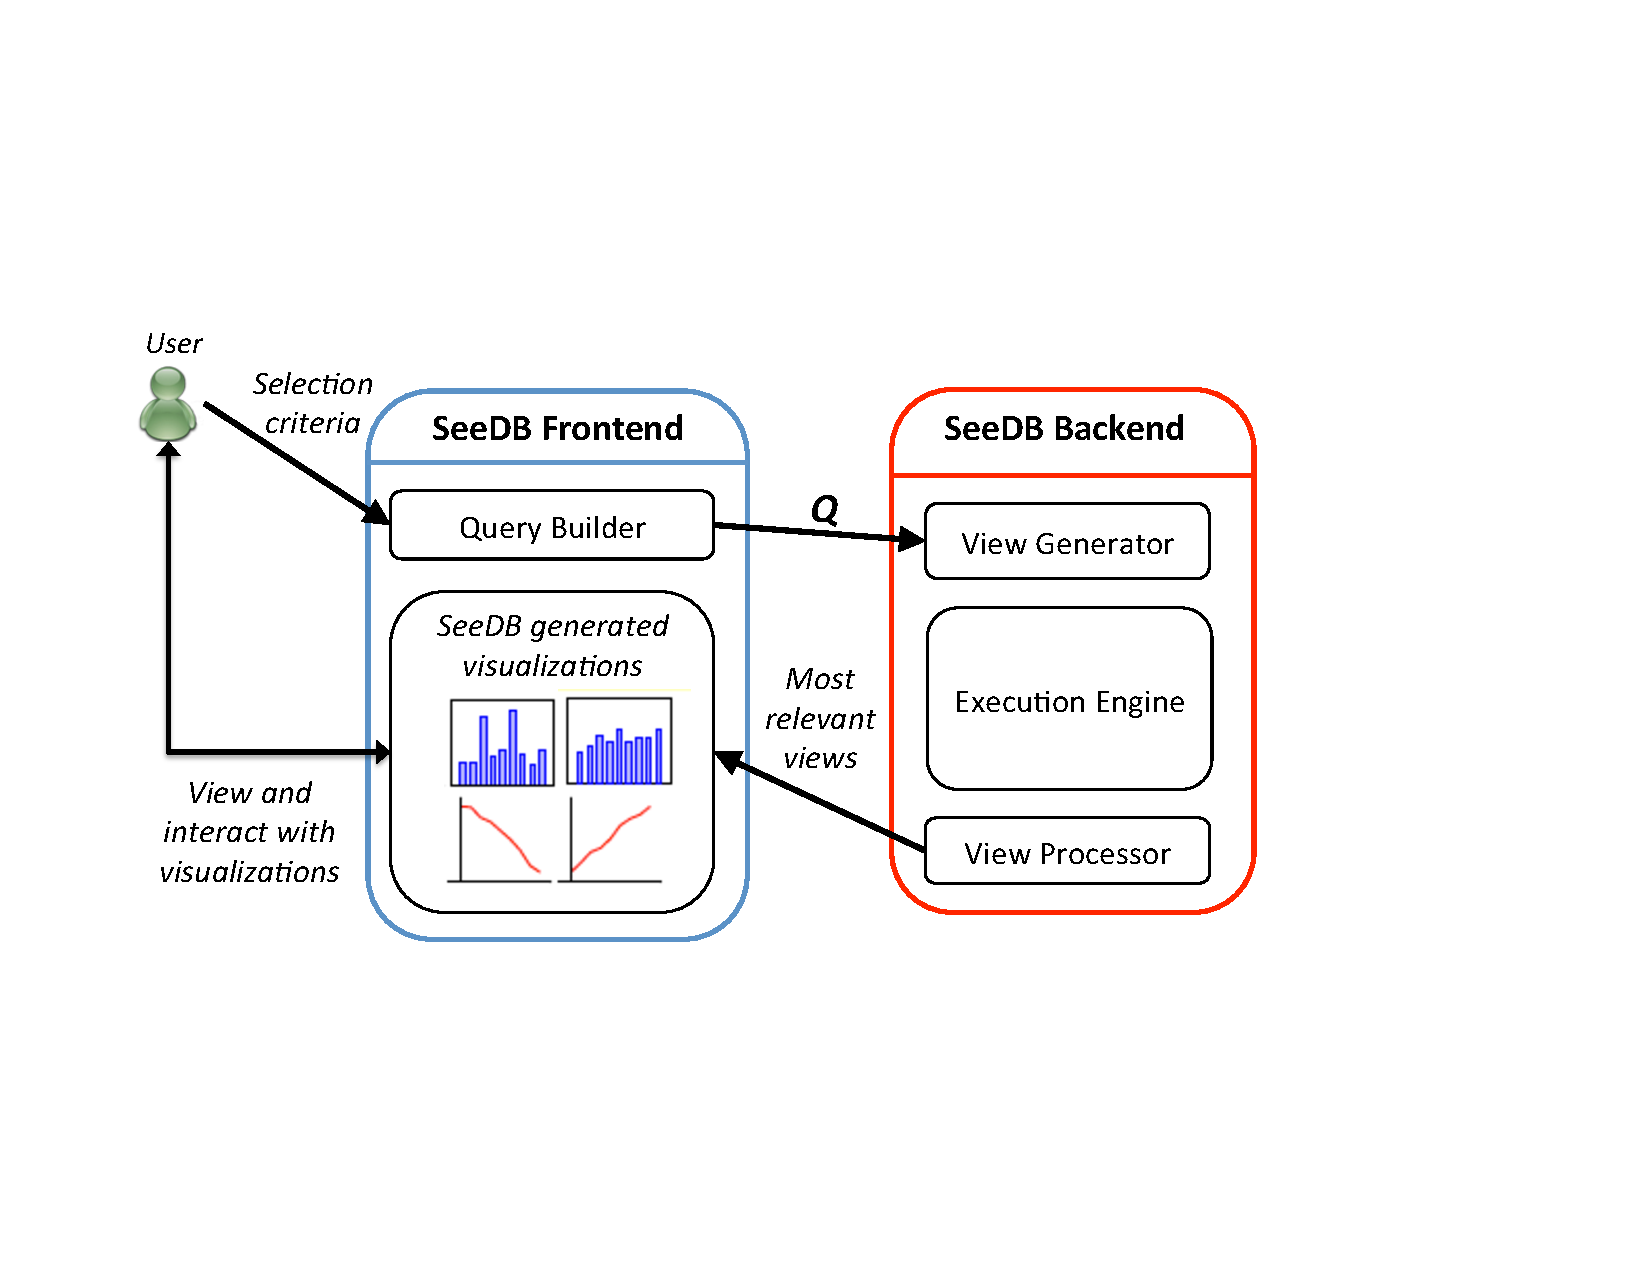
\includegraphics[trim=10mm 45mm 55mm 60mm, 
clip=true]{Images/seedb-architecture.pdf}}}}
\caption{SeeDB Architecture}
\label{fig:sys-arch}
\vspace{-12pt}
\end{figure} 

In this work, we explored two distinct implementations of the \SeeDB\ Execution
Engine. 
First, we built the Execution Engine as a wrapper on top of a database system. 
Our goal was to study how far we could push existing systems to support a
\SeeDB-type workload.
As described in the next section, we could get reasonable performance by
intelligently combining queries and running queries in parallel. 
However, existing systems do not provide a good means to share scans between
queries or to access intermediate results during scans.
As a result, optimization opportunities are limited.
To overcome the constraints of existing database systems, we then implemented a
simple, custom Execution Engine for \SeeDB\ that was optimized to share scans
across all views and perform pruning based on intermediate results. 
In an ideal solution, shared scans and pruning would be implemented inside the
database; however, for the purpose of this work, we implement the \SeeDB\
execution engine as a standalone component. 
In Section \ref{} we discuss how the \SeeDB\ engine could be made part of a
DBMS.

Next we briefly examine the \SeeDB\ frontend and describe the Execution Engines
in detail.


% In the DBMS-based execution engine (Section \ref{}), the view stubs are passed
% through the optimizer that identifies the best ways to combine the queries to minimize
% execution time.
% Once the views have been optimized, the views are rewritten as SQL queries and
% executed against the underlying database. 
% The results of these queries are
% processed to update the view stubs and compute view utility. 
% Once all the queries have been processed, the top-k views are returned to the
% frontend.
% 
% In the main-memory execution engine, \SeeDB\ makes a single pass through the
% data (either read from disk or already present in memory) and keeps running
% estimates of utility for each of the views stubs obtained from the View
% Generator. 
% As the engine processes more of the data, the utility estimates become more
% accurate and \SeeDB\ uses various pruning heuristics to prune out views on the fly.
% By the time the full data has been processed, \SeeDB\ has identified the top-k
% views with the largest utility that are then returned to the frontend.


